\documentclass[11pt,a4paper]{article}

\usepackage[utf8]{inputenc}
\usepackage[T1]{fontenc}
\usepackage[margin=2.5cm]{geometry}
\usepackage{graphicx}
\usepackage{booktabs}
\usepackage{amsmath,amssymb}
\usepackage{caption}
\usepackage{microtype}
\usepackage{tikz}
\usetikzlibrary{positioning,arrows.meta}
\usepackage[colorlinks=true,linkcolor=blue,citecolor=blue,urlcolor=blue]{hyperref}

\graphicspath{{figures/}{architecture/}}

\title{Learning to Anticipate: LSTM Hand-Trajectory Prediction for
       Latency Compensation in Vision-Based Robot Teleoperation}
\author{Your Name\\ \small Machine Learning --- Final Project, NTNU}
\date{June 2026}

\begin{document}
\maketitle

\begin{abstract}
We extend a working vision-based teleoperation system---MediaPipe hand tracking
driving a 6-DOF robot arm through MoveIt Servo pose tracking---with a learned
trajectory predictor. The existing pipeline smooths the noisy hand position with
an exponential moving average (EMA), which trades jitter for lag: the robot is
always commanded toward where the hand \emph{was}. We replace this with a small
LSTM (4.7k parameters) trained on 22{,}420 self-collected hand positions to
predict the hand's position $\sim$100\,ms \emph{ahead}, compensating the
camera--inference--control latency. A first formulation that regressed absolute
coordinates failed dramatically (10.6\,mm test MAE, losing to a trivial
copy-last-frame baseline at 0.8\,mm) due to distribution shift between
workspace regions under a leakage-safe chronological split; reformulating the
task as translation-invariant \emph{displacement} prediction fixed it. The
final model achieves 2.32\,mm MAE and 5.68\,mm RMSE at a 98\,ms prediction horizon,
outperforming the persistence baseline (4.36\,mm MAE) by 47\% and the deployed EMA
pipeline (7.20\,mm MAE) by 68\%; the RMSE ratio is even more favourable ($2.9{\times}$
vs.\ the EMA). Under 5-fold blocked cross-validation the LSTM scores
$2.28 \pm 0.45$\,mm MAE and $4.75 \pm 1.67$\,mm RMSE, beating both baselines in every
fold on both metrics. The model is exported to TorchScript and runs
inside the live teleoperation node at 0.2\,ms per inference with a runtime
LSTM/EMA toggle for A/B comparison. On the real robot the improvement in the
target signal is measurable but not perceptible, which we attribute to the
system being actuator-limited rather than perception-limited; we analyze this
honestly as a system-level negative result.
\end{abstract}

\section{Introduction}

Vision-based teleoperation lets an operator control a robot arm with bare-hand
motion captured by a single webcam. Our existing system (built prior to this
project) tracks the operator's right hand with MediaPipe Hands, maps the hand
position to a target end-effector pose, and servos a 6-DOF arm toward that
target with MoveIt Servo's pose-tracking controller. The system works, but the
raw hand position estimated from camera images is noisy---landmark jitter,
camera noise, and a hand-size-based depth estimate all contribute---so the
pipeline smooths it with an exponential moving average (EMA). Smoothing
introduces the classic tradeoff: the smoother the output, the more it
\emph{lags} the true hand position, so the robot is always chasing a point
behind the operator's hand.

From a machine learning perspective, this lag is a forecasting problem. If a
model can predict where the hand \emph{will be} a few frames from now, the
pipeline can command the predicted position instead of a delayed estimate,
converting lag into lead. Hand motion is highly structured---velocities persist,
trajectories curve smoothly---so a short history window carries real predictive
signal. Predictive latency compensation of this kind is an established idea in
telerobotics; the contribution here is a complete, self-contained
implementation and honest evaluation of it on our own system.

Concretely, this project contributes:
\begin{enumerate}
  \item a data-collection mode built into the teleoperation node that records
        raw and EMA-smoothed hand trajectories to CSV (22{,}420 samples
        collected over two sessions);
  \item a self-supervised problem formulation---predicting hand
        \emph{displacement} $H$ frames ahead from a window of past
        positions---including the failure analysis that motivated it
        (Section~\ref{sec:failure});
  \item a leakage-safe evaluation against two baselines (persistence and the
        deployed EMA), with a 47\%/68\% error reduction respectively;
  \item deployment of the trained model in the live ROS\,2 node via
        TorchScript, with a runtime A/B toggle and a replay-based
        verification that the deployed code path bit-reproduces the offline
        evaluation;
  \item a candid system-level analysis of why the measured signal improvement
        does not (yet) translate into a perceptibly better teleoperation feel.
\end{enumerate}

\section{Background}
\label{sec:background}

This section briefly introduces the three pre-existing components the project
builds on: the hand tracker that produces our input signal, and the
servoing/control stack that consumes our output.

\subsection{MediaPipe Hands}

MediaPipe Hands~\cite{mediapipe} is Google's pre-trained, on-device hand
tracker. It is a two-stage pipeline (Figure~\ref{fig:mediapipe}): a palm
\emph{detector} locates the hand in the full frame, and a landmark CNN then
regresses 21 3-D hand landmarks from the cropped hand region. The expensive
detector does \emph{not} run every frame---only on the first frame or when the
hand is lost; otherwise the landmarks of frame $t$ define the crop for frame
$t{+}1$ (the temporal back edge in the figure), which is what makes 30\,Hz
tracking feasible on CPU. We use this network frozen, purely as a feature
extractor: the wrist landmark gives the image-plane position, the
wrist-to-knuckle distance gives the depth cue, and fingertip configurations
drive the gripper gestures. The landmark jitter inherent in per-frame CNN
regression is one of the noise sources our predictor must cope with.

\begin{figure}[t]
  \centering
  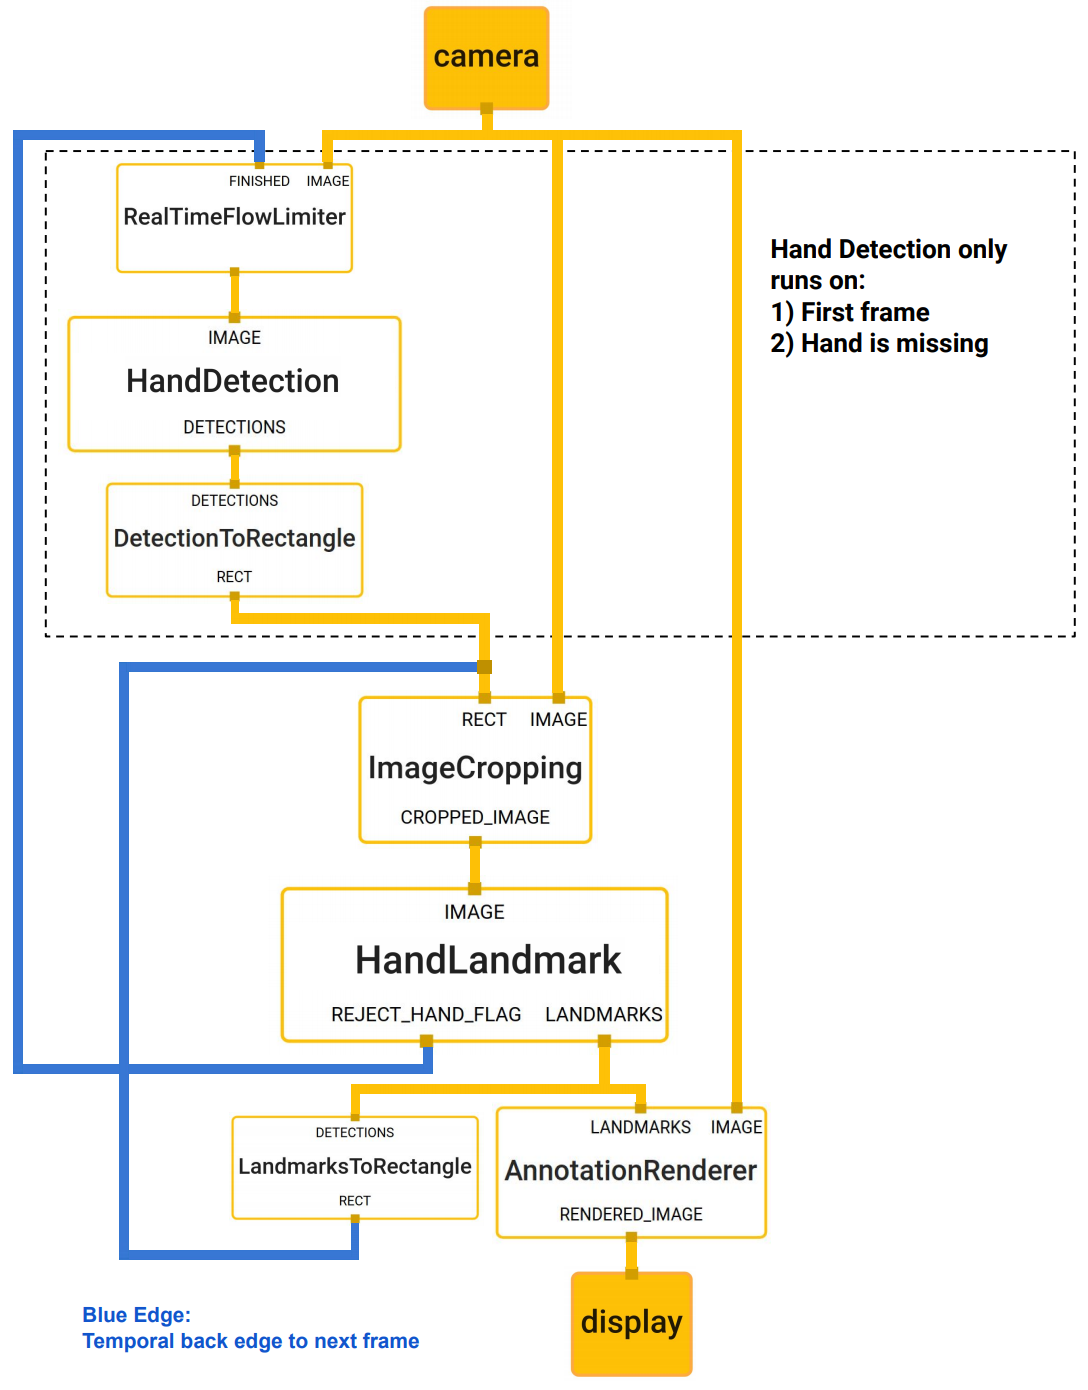
\includegraphics[width=.55\linewidth]{mediapipe}
  \caption{MediaPipe Hands dataflow: palm detection runs only when tracking is
           lost; the landmark model otherwise tracks frame-to-frame via the
           temporal back edge (blue). Figure reproduced from the official
           MediaPipe documentation~\cite{mediapipe}.}
  \label{fig:mediapipe}
\end{figure}

\subsection{MoveIt Servo and Pose Tracking}

Classical MoveIt operation is \emph{plan-then-execute}: compute a full
trajectory to a goal, then run it. That is unsuitable for teleoperation, where
the goal moves continuously. MoveIt Servo~\cite{servo} instead consumes a
stream of Cartesian velocity (twist) commands and converts them, at a fixed
rate, into joint commands via differential inverse kinematics,
$\dot{\mathbf{q}} = J^{\dagger}(\mathbf{q})\,\mathbf{v}$, where $J^{\dagger}$
is the pseudo-inverse of the manipulator Jacobian. Around this core, Servo
enforces joint position/velocity limits, scales velocities down near
singularities, checks collisions, and low-pass-filters the output.

\emph{Pose tracking} is a thin control layer on top of Servo: a proportional
controller computes the error between the current end-effector pose (from
joint states via forward kinematics) and the target pose on
\texttt{/hand\_target\_pose}, and emits the corrective twist that Servo
executes. Our C++ tracking node runs this in \emph{position-only} mode: the
orientation error is ignored, because a 6-DOF arm has no kinematic redundancy
(no null space), so simultaneously forcing position and a fixed orientation
over a large workspace drives the wrist into joint limits. Note the
feedback loop is closed on \emph{joint encoders}, not on vision: the camera
only generates the reference, which distinguishes this architecture from
visual servoing.

\subsection{Execution Layer: ros2\_control}

Figure~\ref{fig:ros2control} shows where everything lands. MoveIt (and our
Servo node) are \emph{third-party} layers that ultimately publish to
controllers managed by ros2\_control~\cite{ros2control}: in our setup, Servo's
output feeds a \texttt{JointTrajectoryController} (\texttt{arm\_controller}),
which streams position references through the hardware interface to the arm's
serial-bus servo motors; a parallel \texttt{GripperActionController} drives
the gripper. The same controller graph runs unmodified against mock hardware,
which is how the system (and this project's predictor) was tested in
simulation before touching the robot.

\begin{figure}[t]
  \centering
  
\includegraphics[width=.95\linewidth]{moveit}
  \caption{The ROS\,2 control stack: MoveIt\,2 sits above ros2\_control's
           controller manager and hardware interfaces. Diagram by D.~\v{S}togl
           and B.~Magyar (ros2\_control project), CC-BY~\cite{ros2control}.}
  \label{fig:ros2control}
\end{figure}

\section{System Overview}
\label{sec:system}

Figure~\ref{fig:pipeline} shows the pipeline. A webcam frame is processed by
MediaPipe Hands, a pre-trained network that returns 21 hand landmarks. The
wrist position in the image gives lateral/vertical coordinates; the apparent
palm length (wrist to middle-finger knuckle) provides a monotonic depth cue.
These are affinely mapped into a workspace box in the robot's planning frame,
yielding a raw 3-D target position $\mathbf{p}_t \in \mathbb{R}^3$ at
$\sim$30\,Hz. The existing pipeline smooths this with an EMA,
\begin{equation}
  \mathbf{s}_t = (1-\alpha)\,\mathbf{s}_{t-1} + \alpha\,\mathbf{p}_t,
  \qquad \alpha = 0.3,
  \label{eq:ema}
\end{equation}
whose group delay of roughly $(1-\alpha)/\alpha \approx 2.3$ frames
($\approx$75\,ms at 30\,Hz) is the lag this project targets. The published
target pose is consumed by a C++ MoveIt Servo node that runs a proportional
controller on the pose error and streams joint commands to the arm. Finger
gestures control the gripper and a named ``ready''-pose reset; both are
unchanged by this project.

\begin{figure}[t]
  \centering
  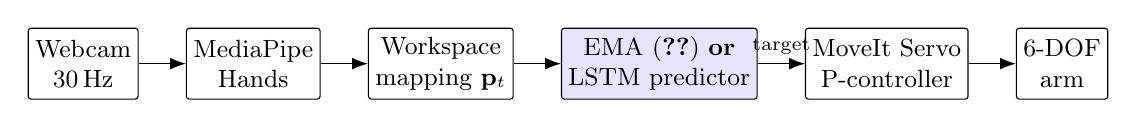
\begin{tikzpicture}[
      node distance=4mm and 6mm,
      box/.style={draw, rounded corners=1pt, align=center,
                  minimum height=9mm, inner sep=2.5pt, font=\small},
      ml/.style={box, fill=blue!10},
      >={Latex[length=2mm]}]
    \node[box]                    (cam)  {Webcam\\ 30\,Hz};
    \node[box, right=of cam]      (mp)   {MediaPipe\\ Hands};
    \node[box, right=of mp]       (map)  {Workspace\\ mapping $\mathbf{p}_t$};
    \node[ml,  right=of map]      (pred) {EMA \eqref{eq:ema} \textbf{or}\\ LSTM predictor};
    \node[box, right=of pred]     (servo){MoveIt Servo\\ P-controller};
    \node[box, right=of servo]    (arm)  {6-DOF\\ arm};
    \draw[->] (cam) -- (mp);
    \draw[->] (mp) -- (map);
    \draw[->] (map) -- (pred);
    \draw[->] (pred) -- node[above, font=\scriptsize]{target} (servo);
    \draw[->] (servo) -- (arm);
  \end{tikzpicture}
  \caption{Teleoperation pipeline. This project replaces the EMA smoothing
           stage (blue) with an LSTM that predicts the hand position
           $\sim$100\,ms ahead; a runtime toggle switches between the two.}
  \label{fig:pipeline}
\end{figure}

\section{Data Collection}
\label{sec:data}

We added a recording mode to the teleoperation node: pressing a key starts
appending one CSV row per tracked frame, containing a monotonic timestamp, a
\emph{segment id}, the raw mapped position $\mathbf{p}_t$, and the EMA output
$\mathbf{s}_t$. The segment id increments whenever hand tracking is lost, so
that no training window is ever built across a tracking gap. Recording the EMA
alongside the raw signal lets us evaluate the deployed smoother as a baseline
on exactly the same frames. The robot does not need to be running; only the
webcam and the tracking node are involved.

We recorded two sessions totalling \textbf{22{,}420 samples}
($\approx$12.3 minutes of tracked motion) in 7 segments at a median frame
interval of 32.8\,ms ($\approx$30\,Hz). The first session ($\sim$3.7\,min)
contained mostly slow, smooth motion (median frame-to-frame displacement
2.9\,mm); the second ($\sim$8.6\,min) was deliberately recorded with mixed
speeds, sweeps, curves, holds, and sharp direction changes (median 3.4\,mm,
99th percentile 33\,mm per frame). Figure~\ref{fig:data} shows a sample of the
raw signal and its EMA.

\begin{figure}[t]
  \centering
  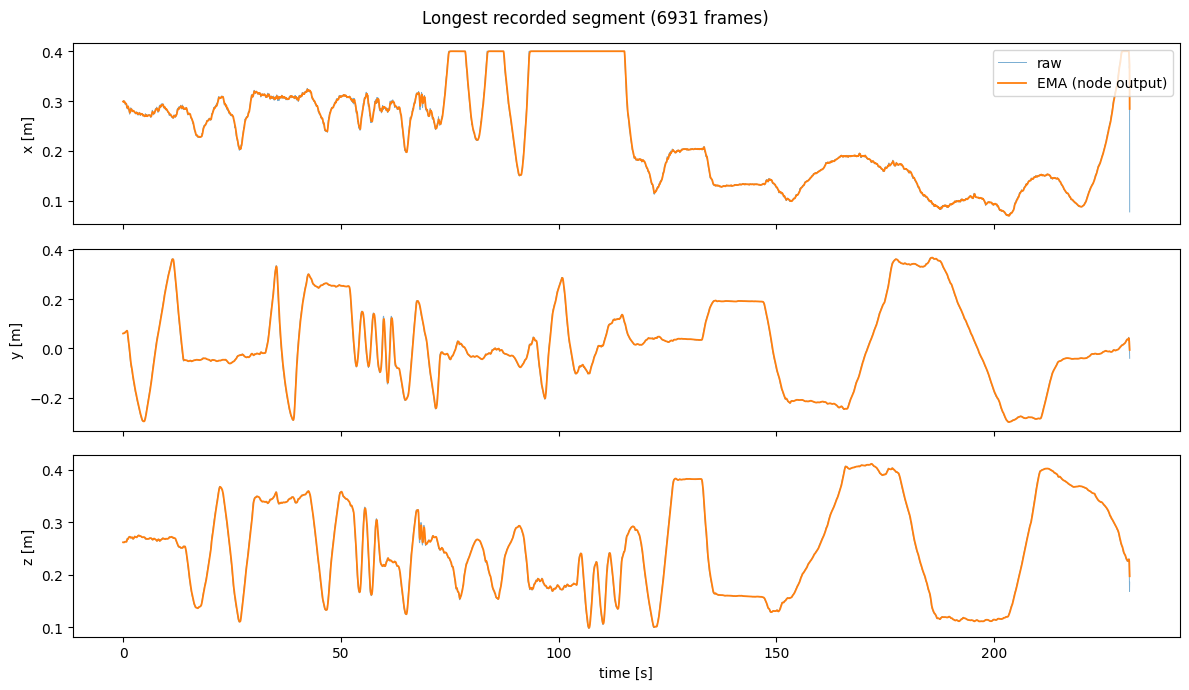
\includegraphics[width=.95\linewidth]{data_overview}
  \caption{A slice of the recorded data: raw mapped hand position (noisy) and
           the node's EMA output (smooth but lagging).}
  \label{fig:data}
\end{figure}

\section{Problem Formulation}
\label{sec:formulation}

\paragraph{Self-supervised forecasting.} No manual labels are required: the
target for each window is simply the position that occurs later in the same
recording. With window length $L=15$ and horizon $H=3$ frames
($\approx$98\,ms at 30\,Hz), every recorded frame contributes automatically to
many training pairs, yielding 22{,}085 windows from 22{,}420 frames.

\paragraph{Displacement (residual) prediction.} The model input is the window
\emph{relative to its last frame}, and the target is the \emph{displacement}
from that frame to the future position:
\begin{equation}
  X_t = \bigl(\mathbf{p}_{t-L+1}-\mathbf{p}_t,\ \dots,\
              \mathbf{p}_{t-1}-\mathbf{p}_t,\ \mathbf{0}\bigr),
  \qquad
  \mathbf{y}_t = \mathbf{p}_{t+H}-\mathbf{p}_t .
  \label{eq:residual}
\end{equation}
The absolute prediction is reconstructed as
$\hat{\mathbf{p}}_{t+H} = \mathbf{p}_t + \hat{\mathbf{y}}_t$. This makes the
model \emph{translation-invariant}: a leftward sweep produces identical
input/target pairs anywhere in the workspace. Section~\ref{sec:failure} shows
empirically why this matters. A useful side effect is that the zero function
reproduces the persistence baseline, so the model starts from a sane default
and only has to learn motion dynamics on top of it. Inputs and targets are
z-normalized with statistics computed on the training split only; the same
constants are exported with the model for deployment.

\paragraph{Model.} A single-layer LSTM with 32 hidden units processes the
window; a linear layer maps the final hidden state to the 3-D displacement:
\begin{equation}
  \mathbf{h}_t = \mathrm{LSTM}(X_t) \in \mathbb{R}^{32},
  \qquad
  \hat{\mathbf{y}}_t = W\mathbf{h}_t + \mathbf{b},
\end{equation}
where the LSTM cell uses the standard gating
\begin{equation}
\begin{aligned}
  \mathbf{i}_k,\mathbf{f}_k,\mathbf{o}_k &=
      \sigma\!\bigl(W_{\{i,f,o\}}[\mathbf{x}_k;\mathbf{h}_{k-1}] + \mathbf{b}_{\{i,f,o\}}\bigr),\qquad
  \mathbf{g}_k = \tanh\!\bigl(W_g[\mathbf{x}_k;\mathbf{h}_{k-1}] + \mathbf{b}_g\bigr),\\
  \mathbf{c}_k &= \mathbf{f}_k \odot \mathbf{c}_{k-1} + \mathbf{i}_k \odot \mathbf{g}_k,\qquad
  \mathbf{h}_k = \mathbf{o}_k \odot \tanh(\mathbf{c}_k).
\end{aligned}
\end{equation}
The full model has $\approx$4{,}700 parameters---deliberately small, since it
must run inside a 30\,Hz control loop and the dataset is modest. Training
minimizes the MSE between $\hat{\mathbf{y}}_t$ and $\mathbf{y}_t$ (both
normalized) with Adam (learning rate $10^{-3}$, batch size 256, 60 epochs),
keeping the parameters of the epoch with the lowest validation loss. Because
the targets contain observation noise, the MSE-optimal predictor approximates
the \emph{conditional mean} of the future position---the network learns to
smooth like the EMA while anticipating instead of lagging.

\paragraph{Leakage-safe evaluation.} Consecutive frames are nearly identical,
so randomly shuffling windows before splitting would place near-duplicates of
test samples in the training set and inflate the test score. Instead, each
tracking segment is split chronologically 70/15/15 into train/validation/test,
and windows are built within each piece so none crosses a split or segment
boundary. We report mean absolute error (MAE) and root-mean-square error
(RMSE) in millimetres in absolute coordinates against the raw position $H$
frames ahead, for three methods:
\begin{itemize}
  \item \textbf{LSTM (ours):} $\mathbf{p}_t + \hat{\mathbf{y}}_t$;
  \item \textbf{Persistence:} $\mathbf{p}_t$ (``the hand will not move''), the
        standard forecasting sanity baseline;
  \item \textbf{EMA (deployed pipeline):} $\mathbf{s}_t$, i.e.\ what the
        existing system would command at prediction time.
\end{itemize}

\section{A Negative Result and Its Fix: Absolute vs.\ Displacement Prediction}
\label{sec:failure}

Our first formulation regressed the \emph{absolute} future position from the
raw (absolute) window. On synthetic data it worked; on the real recording it
failed badly (Table~\ref{tab:failure}, top row): 10.56\,mm test MAE, more than
$12\times$ worse than the trivial persistence baseline.

\begin{table}[t]
  \centering
  \caption{The failure and its fix (first recording session, $H{=}1$,
           identical network and training; errors on the held-out test split).}
  \label{tab:failure}
  \begin{tabular}{lccc}
    \toprule
    Formulation & LSTM MAE & Persistence MAE & EMA MAE \\
    \midrule
    Absolute position      & 10.56\,mm & 0.84\,mm & 2.07\,mm \\
    Displacement \eqref{eq:residual} & \textbf{0.58\,mm} & 0.84\,mm & 2.07\,mm \\
    \bottomrule
  \end{tabular}
\end{table}

The diagnosis is a textbook distribution shift. Under the chronological split,
the test set is the \emph{end} of the session, and the operator had drifted to
a different part of the workspace by then: the training-split mean position
was $(x,y) = (0.27, +0.02)$\,m versus $(0.15, -0.12)$\,m for the test split.
A network that regresses absolute coordinates can interpolate inside the
region it was trained on but cannot extrapolate outside it; its test
predictions were systematically pulled toward the training region, producing a
$\sim$10\,mm bias. Note that ``fixing'' this by shuffling the split would have
hidden the problem behind data leakage rather than solving it---the model
would still have failed in any new workspace region at deployment time.

The displacement formulation~\eqref{eq:residual} removes the failure mode
entirely, because displacements are translation-invariant: the same network
and training procedure then \emph{beat} both baselines (Table~\ref{tab:failure},
bottom row). We consider this failure-diagnosis-fix cycle the most instructive
outcome of the project.

\paragraph{Choosing the horizon.} With the displacement formulation validated,
we swept the prediction horizon on the first session
(Table~\ref{tab:horizon}). At $H{=}1$ (33\,ms) there is little to predict---the
persistence baseline is already nearly perfect on smooth motion. The relative
advantage of learning grows with the horizon, and $H{=}3$ ($\approx$98\,ms)
matches the latency we want to compensate, so we adopt it.

\begin{table}[t]
  \centering
  \caption{Horizon sweep (first session, displacement formulation). MAE in mm.}
  \label{tab:horizon}
  \begin{tabular}{lcccc}
    \toprule
    Horizon (lead time) & LSTM & Persistence & EMA \\
    \midrule
    $H=1$ ($\sim$33\,ms)  & \textbf{0.58} & 0.84 & 2.07 \\
    $H=3$ ($\sim$98\,ms)  & \textbf{1.23} & 1.99 & 3.20 \\
    $H=5$ ($\sim$163\,ms) & \textbf{1.86} & 3.09 & 4.27 \\
    \bottomrule
  \end{tabular}
\end{table}

\section{Results}
\label{sec:results}

The final model was trained on the combined dataset (15{,}573 training,
3{,}255 validation, and 3{,}257 test windows). Figure~\ref{fig:loss} shows the
convergence behaviour: training loss decreases monotonically, while validation
loss reaches its minimum ($0.099$, normalized) around epoch 20 and then drifts
upward---mild overfitting. The best-validation checkpoint selection neutralizes
this: the deployed model is the epoch-20 one, so checkpointing acts as early
stopping and the later epochs are simply discarded. Two further observations:
validation loss sits above training loss throughout, because the chronological
split places somewhat different motion in the validation slices than in the
training slices (a distribution difference, not estimation variance); and
although the window count exceeds the parameter count by $3\times$,
overlapping windows are highly correlated, so the effective sample size is
smaller than the nominal count---consistent with overfitting appearing despite
the seemingly comfortable data-to-parameter ratio.

\begin{figure}[t]
  \centering
  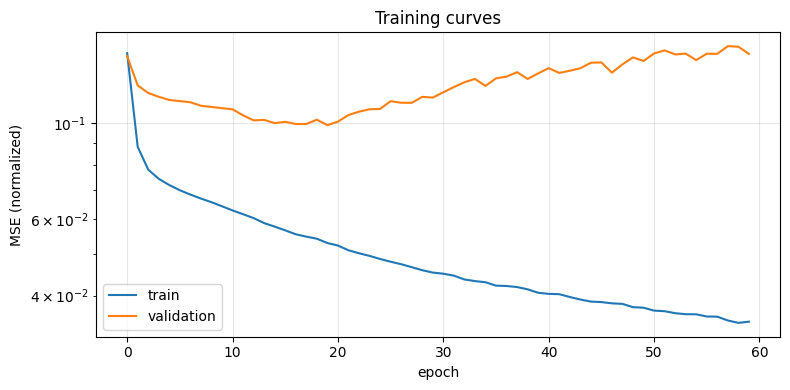
\includegraphics[width=.7\linewidth]{loss_curve}
  \caption{Training and validation loss (MSE, normalized units, log scale).}
  \label{fig:loss}
\end{figure}

\begin{table}[t]
  \centering
  \caption{Test-set error at the 98\,ms prediction horizon, combined dataset.}
  \label{tab:results}
  \begin{tabular}{lccc}
    \toprule
    Method & MAE [mm] & RMSE [mm] & per-axis MAE $[x\ y\ z]$ [mm] \\
    \midrule
    \textbf{LSTM (ours)}     & \textbf{2.32} & \textbf{5.68} & $[2.09\ \ 2.83\ \ 2.04]$ \\
    Persistence (copy last)  & 4.36 & 10.27 & $[2.48\ \ 6.31\ \ 4.29]$ \\
    EMA (deployed pipeline)  & 7.20 & 16.75 & $[3.57\ \ 10.85\ \ 7.19]$ \\
    \bottomrule
  \end{tabular}
\end{table}

Table~\ref{tab:results} gives the headline result: the LSTM reduces the target
error by \textbf{47\%} relative to persistence and \textbf{68\%} relative to
the deployed EMA. The RMSE gap is even larger ($2.9\times$ vs.\ the EMA)
because RMSE emphasizes the large errors that occur during fast motion---
precisely where velocity extrapolation pays off and where the EMA lags most.
Compared with our earlier single-session experiments the absolute errors are
higher, which is expected: the second session deliberately contains fast
motion, making the test set harder for every method (the persistence error
more than doubled). The honest comparison is therefore the relative one, and
it improved with the harder data.

\paragraph{Cross-validation.} A single chronological split yields one test
estimate; to quantify its variance we ran 5-fold \emph{blocked} cross-validation
with purging. Plain $k$-fold is invalid on time series---random folds would
scatter near-duplicate consecutive frames across train and test (the same
leakage the chronological split avoids)---so instead each fold's test set is a
contiguous time block of every segment, the model is retrained from scratch on
the remainder, and a gap of $L{+}H$ frames around each test block is discarded
so that no training window overlaps test frames. Table~\ref{tab:cv} reports both
MAE and RMSE for all five folds. The LSTM achieves $2.28 \pm 0.45$\,mm MAE
($4.75 \pm 1.67$\,mm RMSE) versus $4.25 \pm 0.72$\,mm MAE ($8.19 \pm 1.75$\,mm
RMSE) for persistence and $6.95 \pm 1.05$\,mm MAE ($13.34 \pm 2.52$\,mm RMSE)
for the EMA, and \textbf{outperforms both baselines in 5 of 5 folds on both
metrics}. The RMSE gap is proportionally larger than the MAE gap---consistent
with the single-split results in Table~\ref{tab:results}---because RMSE
penalises the large errors that occur during fast motion more heavily.
The cross-validated MAE mean agrees with the single-split estimate (2.32\,mm),
confirming the headline result is not an artifact of one particular split.

\begin{table}[t]
  \centering
  \caption{5-fold blocked (purged) cross-validation. Upper rows: MAE (mm);
           lower rows: RMSE (mm). Bold = best per fold.}
  \label{tab:cv}
  \begin{tabular}{lccccc|c}
    \toprule
    Method & fold 1 & fold 2 & fold 3 & fold 4 & fold 5 & mean $\pm$ std \\
    \midrule
    \multicolumn{7}{l}{\textit{MAE (mm)}} \\[2pt]
    \textbf{LSTM (ours)} & \textbf{3.16} & \textbf{2.10} & \textbf{1.91} & \textbf{2.08} & \textbf{2.14} & $\mathbf{2.28 \pm 0.45}$ \\
    Persistence          & 5.64 & 4.17 & 3.92 & 3.55 & 3.96 & $4.25 \pm 0.72$ \\
    EMA (deployed)       & 8.92 & 6.91 & 6.61 & 5.78 & 6.53 & $6.95 \pm 1.05$ \\
    \midrule
    \multicolumn{7}{l}{\textit{RMSE (mm)}} \\[2pt]
    \textbf{LSTM (ours)} & \textbf{7.55} & \textbf{3.26} & \textbf{2.87} & \textbf{4.84} & \textbf{5.24} & $\mathbf{4.75 \pm 1.67}$ \\
    Persistence          & 11.05 & 7.07 & 6.39 & 7.07 & 9.37 & $8.19 \pm 1.75$ \\
    EMA (deployed)       & 17.27 & 11.94 & 10.93 & 11.20 & 15.34 & $13.34 \pm 2.52$ \\
    \bottomrule
  \end{tabular}
\end{table}

Figure~\ref{fig:overlay} shows the qualitative behaviour on the longest test
piece: the EMA visibly trails the raw trajectory during motion, while the LSTM
prediction tracks and slightly leads it. Output smoothness (mean
frame-to-frame step) is 0.84\,mm for the raw signal, 0.57\,mm for the EMA, and
1.05\,mm for the LSTM: on this data the raw signal is already smooth, so the
model's benefit is anticipation rather than denoising---had the input been
jitterier, the conditional-mean property of MSE training would also have
smoothed it.

\begin{figure}[t]
  \centering
  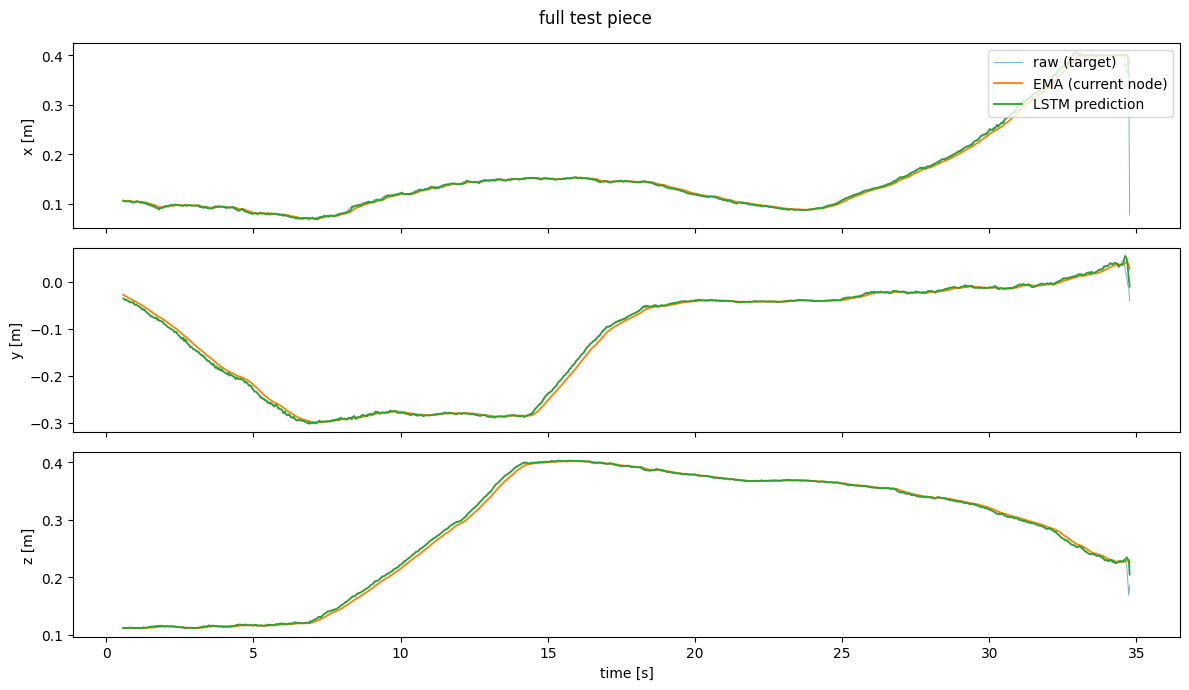
\includegraphics[width=.95\linewidth]{test_full}\\[2mm]
  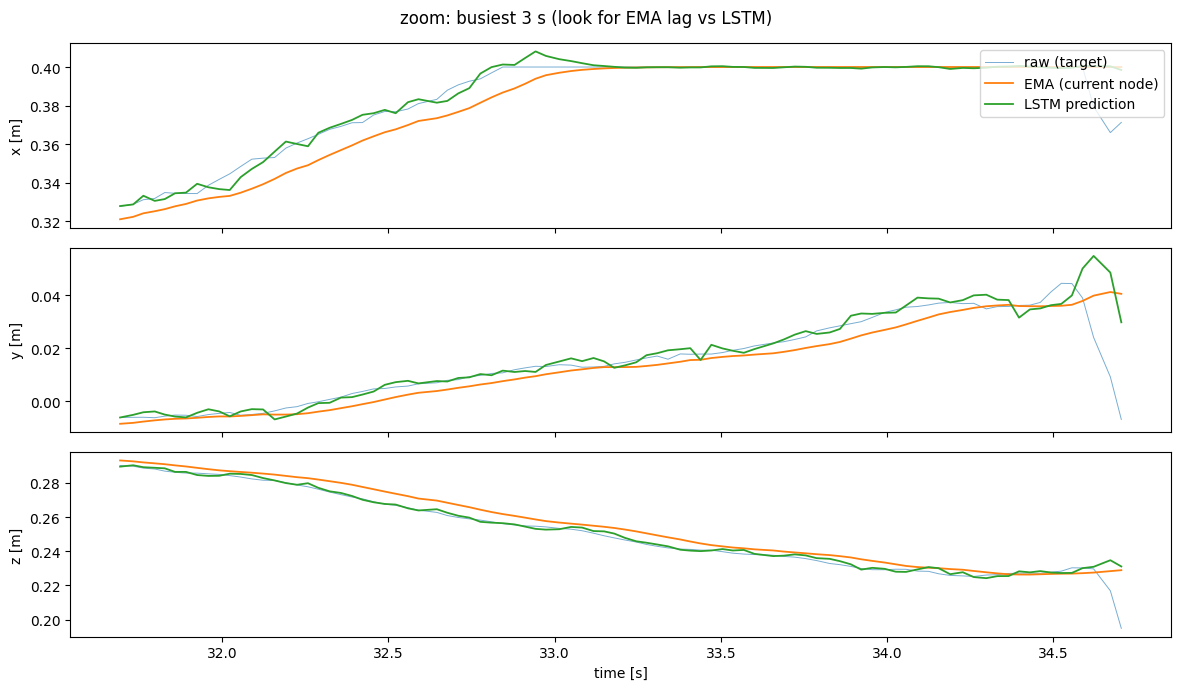
\includegraphics[width=.95\linewidth]{test_zoom}
  \caption{Longest test piece (top) and a zoom on its busiest three seconds
           (bottom): raw target, EMA (lags during motion), and the LSTM
           prediction.}
  \label{fig:overlay}
\end{figure}

\section{Deployment on the Robot}
\label{sec:deployment}

The trained model is exported three ways: a PyTorch state dict (for
retraining), a TorchScript module (loadable without the Python class
definition), and a JSON file with the window configuration and normalization
constants. The teleoperation node loads the TorchScript model at startup and
maintains a ring buffer of the last $L{=}15$ raw positions. Once the buffer is
full, the published target becomes the clamped LSTM prediction
$\mathbf{p}_t + \hat{\mathbf{y}}_t$; while the buffer fills ($\approx$0.5\,s
after the hand appears), after any tracking loss (which clears the buffer), or
if the model files are missing, the node falls back to the EMA. Predictions
are clamped to the configured workspace box so the model can never command a
pose outside the safety limits. A keyboard toggle switches between LSTM and
EMA at runtime for A/B comparison, with the active mode shown in the camera
overlay.

Deployment was verified without hardware by replaying the recorded CSVs
through the node's exact prediction code path: the replayed test-region MAE
matched the notebook evaluation to within 0.01\,mm, confirming that
normalization, windowing, and reconstruction are identical between training
and deployment. Inference takes 0.1--0.2\,ms per frame on CPU (after a JIT
warm-up at load time), negligible against the 33\,ms frame budget. The model
trained under PyTorch 2.7 loads and runs unchanged under the deployment
machine's PyTorch 2.11 via TorchScript.

\section{Discussion: A Measurable Signal, an Imperceptible Robot}
\label{sec:discussion}

On the real robot, switching between LSTM and EMA modes produced no
perceptible difference in teleoperation feel, even during fast motion. We
report this candidly and believe the explanation is structural: the target
signal is only the first stage of the latency chain. Downstream, the
proportional pose controller and the arm's velocity and acceleration limits
impose a response lag that is several times larger than the $\sim$100--175\,ms
recovered in the command signal. In control terms, the system is
\emph{actuator-limited}, not perception-limited: improving the fastest stage
of the pipeline is masked by the slowest one. The operator had also adapted to
the original system's latency over a week of use, which further compresses the
subjective difference.

This does not make the predictor useless---it makes its benefit conditional.
The 68\% reduction in target error is real and would translate into felt
improvement on a platform with higher control bandwidth (a faster arm, a
stiffer controller, or higher servo gains), or in applications where the
command signal is used directly (e.g.\ logging, shared autonomy, or collision
checking ahead of the robot's motion). For this platform, the honest claim is:
the predictor measurably improves the reference the robot is asked to track,
and the robot is currently the bottleneck in exploiting it.

\section{Limitations and Future Work}
\label{sec:limitations}

\begin{itemize}
  \item \textbf{Data diversity, not data volume.} Validation behaviour shows
        22k samples suffice for a 4.7k-parameter model, but all data come from
        one operator, one camera, and two sessions. Generalization across
        users and lighting conditions is untested.
  \item \textbf{Within-dataset validation only.} Blocked cross-validation
        (Table~\ref{tab:cv}) bounds the split-to-split variance, but all folds
        still come from the same two recording sessions; it cannot measure
        generalization to a new user or camera setup.
  \item \textbf{Baselines.} A Kalman filter with a constant-velocity model is
        the natural classical competitor and would sharpen the claim about
        what the LSTM adds beyond linear extrapolation.
  \item \textbf{System-level evaluation.} A quantitative end-to-end comparison
        (recording the commanded target and the actual end-effector pose in
        both modes during scripted fast motions) would replace the subjective
        ``feels the same'' with a measured tracking-error curve, and would
        directly test the actuator-limited hypothesis.
  \item \textbf{Extensions.} Velocity input features, longer horizons with
        uncertainty estimates, or training across multiple operators.
\end{itemize}

\section{Conclusion}

We turned a latency problem in a working vision-based teleoperation system
into a supervised learning problem, collected our own dataset, and trained a
deliberately small LSTM to predict hand displacement $\sim$100\,ms ahead. A
failed first formulation (absolute-coordinate regression) was diagnosed as
distribution shift under a leakage-safe split and fixed by a
translation-invariant reformulation---after which the model beat both the
persistence baseline (by 47\%) and the deployed EMA pipeline (by 68\%) on
held-out data, and ran in real time on the robot with a verified
training-to-deployment match. The system-level effect is currently masked by
actuator dynamics, which we analyze as an honest negative result: the
predictor improves the reference signal; exploiting it fully requires a faster
plant.

\appendix
\section{Reproducibility}

All code, data, and the trained model are in the
\texttt{mediapipe\_dual\_arm\_control} ROS\,2 package
(branch \texttt{final\_project}):
\begin{itemize}
  \item \texttt{scripts/hand\_pose\_publisher\_node.py} --- teleoperation node
        with the recording mode (\texttt{r} key), the deployed LSTM predictor,
        and the LSTM/EMA toggle (\texttt{m} key);
  \item \texttt{dataset/hand\_traj\_*.csv} --- the recorded sessions
        (22{,}420 frames);
  \item \texttt{notebooks/train\_lstm\_hand\_trajectory.ipynb} --- the full
        pipeline: loading, splitting, training, evaluation, figures, export
        (PyTorch 2.7, executed end-to-end);
  \item \texttt{models/lstm\_hand\_traj.\{pth, torchscript.pt, json\}} --- the
        trained model and its normalization constants.
\end{itemize}
Workflow: run the node (robot optional), press \texttt{r} and move the hand to
record; run all notebook cells to retrain and re-export; restart the node to
deploy the new model. Hyperparameters: $L{=}15$, $H{=}3$, hidden size 32, one
layer, Adam ($10^{-3}$), batch 256, 60 epochs, best-validation checkpoint,
seed 42.

\begin{thebibliography}{9}

\bibitem{mediapipe}
F.~Zhang, V.~Bazarevsky, A.~Vakunov, A.~Tkachenka, G.~Sung, C.-L.~Chang, and
M.~Grundmann, ``MediaPipe Hands: On-device Real-time Hand Tracking,''
\emph{arXiv:2006.10214}, 2020.
\url{https://ai.google.dev/edge/mediapipe/solutions/vision/hand_landmarker}

\bibitem{servo}
PickNik Robotics / MoveIt maintainers, ``MoveIt Servo --- Real-time Arm
Servoing,'' \emph{MoveIt\,2 Documentation}, 2024.
\url{https://moveit.picknik.ai/humble/doc/examples/realtime_servo/realtime_servo_tutorial.html}

\bibitem{ros2control}
D.~\v{S}togl, B.~Magyar, et~al., ``ros2\_control: A Generic and Composable
Framework for Real-Time Robot Control,'' \emph{ros2\_control Documentation},
2024. \url{https://control.ros.org}

\end{thebibliography}

\end{document}
